\documentclass{article}

\usepackage{fancyhdr} % Required for custom headers
\usepackage{lastpage} % Required to determine the last page for the footer
\usepackage{extramarks} % Required for headers and footers
\usepackage[usenames,dvipsnames]{color} % Required for custom colors
\usepackage{graphicx} % Required to insert images
\usepackage{listings} % Required for insertion of code
\usepackage{courier} % Required for the courier font
\usepackage{lipsum} % Used for inserting dummy 'Lorem ipsum' text into the template
\usepackage{hyperref}
\usepackage{multirow}
\usepackage{tabularx}
\usepackage{framed}
\usepackage{longtable}
\usepackage{listings}
\usepackage{subfigure}
\usepackage{afterpage}
\usepackage{amsmath,amssymb}            
\usepackage{rotating}  
\usepackage{fancyhdr}
\usepackage{graphicx}
\usepackage{amsthm}
\usepackage[scriptsize]{caption} 
\hyphenation{a-gen-tiz-za-zio-ne}
% Margins
\topmargin=-0.45in
\evensidemargin=0in
\oddsidemargin=0in
\textwidth=6.5in
\textheight=9.0in
\headsep=0.25in

\linespread{1.1} % Line spacing

\lstset{
  numbers=left,
  stepnumber=5,    
  firstnumber=1,
  numberfirstline=true
}

% Set up the header and footer
\pagestyle{fancy}
\lhead{\hmwkAuthorName} % Top left header
\chead{\hmwkClass\ (\hmwkClassInstructor\ \hmwkClassTime): \hmwkTitle} % Top center head
\rhead{\firstxmark} % Top right header
\lfoot{\lastxmark} % Bottom left footer
\cfoot{} % Bottom center footer
\rfoot{Page\ \thepage\ of\ \protect\pageref{LastPage}} % Bottom right footer
\renewcommand\headrulewidth{0.4pt} % Size of the header rule
\renewcommand\footrulewidth{0.4pt} % Size of the footer rule

\setlength\parindent{0pt} % Removes all indentation from paragraphs

\usepackage{listings}
\usepackage{color}

\definecolor{dkgreen}{rgb}{0,0.6,0}
\definecolor{gray}{rgb}{0.5,0.5,0.5}
\definecolor{mauve}{rgb}{0.58,0,0.82}

\lstset{frame=tb,
  language=Java,
  aboveskip=3mm,
  belowskip=3mm,
  showstringspaces=false,
  columns=flexible,
  basicstyle={\small\ttfamily},
  numbers=none,
  numberstyle=\tiny\color{gray},
  keywordstyle=\color{blue},
  commentstyle=\color{dkgreen},
  stringstyle=\color{mauve},
  breaklines=true,
  breakatwhitespace=true
  tabsize=3
}

%----------------------------------------------------------------------------------------
%	DOCUMENT STRUCTURE COMMANDS
%	Skip this unless you know what you're doing
%----------------------------------------------------------------------------------------

% Header and footer for when a page split occurs within a problem environment
\newcommand{\enterProblemHeader}[1]{
\nobreak\extramarks{#1}{#1 continued on next page\ldots}\nobreak
\nobreak\extramarks{#1 (continued)}{#1 continued on next page\ldots}\nobreak
}

% Header and footer for when a page split occurs between problem environments
\newcommand{\exitProblemHeader}[1]{
\nobreak\extramarks{#1 (continued)}{#1 continued on next page\ldots}\nobreak
\nobreak\extramarks{#1}{}\nobreak
}




%----------------------------------------------------------------------------------------
%	NAME AND CLASS SECTION
%----------------------------------------------------------------------------------------

\newcommand{\hmwkTitle}{Inheritance and interfaces} % Assignment title
\newcommand{\hmwkDueDate}{Martedi,\ Aprile 15,\ 2014} % Due date
\newcommand{\hmwkClass}{Ingegneria del Software 1} % Course/class
\newcommand{\hmwkClassTime}{} % Class/lecture time
\newcommand{\hmwkClassInstructor}{Carlo Ghezzi} % Teacher/lecturer
\newcommand{\hmwkAuthorName}{} % Your name

%----------------------------------------------------------------------------------------
%	TITLE PAGE
%----------------------------------------------------------------------------------------

\title{
\vspace{2in}
\textmd{\textbf{\hmwkClass:\ \hmwkTitle}}\\
\normalsize\vspace{0.1in}\small{Due\ on\ \hmwkDueDate}\\
\vspace{0.1in}\large{\textit{\hmwkClassInstructor\ \hmwkClassTime}}
\vspace{3in}
}

\author{\textbf{\hmwkAuthorName}}
\date{} % Insert date here if you want it to appear below your name

%----------------------------------------------------------------------------------------

\begin{document}

\maketitle

%----------------------------------------------------------------------------------------
%	TABLE OF CONTENTS
%----------------------------------------------------------------------------------------

%\setcounter{tocdepth}{1} % Uncomment this line if you don't want subsections listed in the ToC

\newpage
\tableofcontents
\newpage



\section{Introduction}

\subsection{HashCode and Equals}
I metodi \texttt{hashCode()} e \texttt{equals()} sono molto utilizzati nella programmazione a oggetti. In particolare:
\begin{itemize}
\item \texttt{hashCode()} la funzione hash \`e una funzione non iniettiva (e quindi non invertibile) che mappa una oggetto in una intero in genere \`e opportuno che l'algoritmo di hashing soddisfi le seguenti caratteristiche
\begin{itemize}
\item quando \`e invocato pi\`u di una volta sullo stesso oggetto deve ritornare lo stesso intero. (Questo intero potrebbe essere diverso in esecuzioni diverse dell'applicazione, l'importante \`e che all'interno di un esecuzione sia sempre lo stesso)
\item se due oggetti sono uguali con riferimento al metodo \texttt{equals} allora  il metodo \texttt{hashCode} deve ritornare lo stesso intero
\item non \`e richiesto che due oggetti non uguali in termini del metodo \texttt{equals} siano associati due \texttt{hashCode} diversi. Tuttavia, il programmatore deve sapere che produrre interi differenti pu\`o migliorare le performances, (per esempio delle hashTables).
\end{itemize}
\item \texttt{equals()} specifica quando un oggetto \`e uguale all'oggetto corrente. Il metodo \texttt{equals} implementa una relazione di equivalenza su degli elementi non nulli. La relazione deve essere
\begin{itemize}
\item \emph{riflessiva} per ogni reference \texttt{x} non nullo \texttt{x.equals(x)} ritorna \texttt{true}
\item \emph{symmetrica} per ogni references \texttt{x} e \texttt{y} non nulli \texttt{x.equals(y)} deve ritornare \texttt{true} se e solo se \texttt{y.equals(x)} ritorna \texttt{true}
\item \emph{transitiva} per ogni \texttt{x}, \texttt{y}, \texttt{z} non nulli se \texttt{x.equals(y)} ritorna true, e \texttt{y.equals(z)} ritorna true allora \texttt{x.equals(z)} deve ritornare \texttt{true}.
\item \emph{consistente}: per ogni \texttt{x} e \texttt{y} non nulli, invocazioni multiple di \texttt{x.equals(y)} devono ritornare consistentemente \texttt{true} o consistentemente \texttt{false} se nessuna informazione utilizzata nel metodo \texttt{equals} \`e modificato.
\item per ogni reference \texttt{x} non nullo, \texttt{x.equals(null)} dovrebbe ritornare \texttt{false}
\end{itemize}
\end{itemize}

\subsection{Auto-boxing e auto-unboxing}
\emph{Auto-boxing}: convertire automaticamente un valore primitivo nel corrispondente oggetto.\\
\emph{Auto-unboxing}: convertire un oggetto in un tipo primitivo.

\subsection{Generici}
I generici consentono di avere \texttt{tipi} come parametri di una vostra classe. Sono differenti dai parametri ``normali" dei metodi che specificano il tipo di una varibile. Usando \emph{classi} e \emph{metodi} generici \`e possibile eseguire le medesime operazioni su \textbf{tipi} di dato diverso. Per esempio immaginiamo di voler scrivere un metodo che stampa un array di \texttt{Bike} e un array di \texttt{Persone}; utilizzando gli elementi descritti fino a questo punto dovreemmo dichiarare due metodi diversi, che considerano due tipi array diverso per eseguire le medesime operazioni, oppure usando un array di Object, non consentendo di specificare che in un caso l'array deve contenere \texttt{Bike} e nell'altro \texttt{Persone}. Non c'\`e modo di specificare che in In altre parole la differenza tra usare i parametri normali e i generici, sono che nel primo caso i parametri rappresentano il \emph{valore} nel secondo il \emph{tipo}.

\`E possibile dichiarare \emph{metodi generici} e \emph{classi generiche}.

Una \emph{classe generica} \`e una classe in cui uno dei suoi attributi \`e parametrizzato mediante un tipo generico. Una classe generica \`e definita attraverso la mediante dichiarazione:

\begin{lstlisting}
class Name<T1, T2, ..., Tn> { /* ... */ }
\end{lstlisting}

dove \texttt{T1}, \texttt{T2}, \texttt{Tn} sono i tipi degli elementi della classe.

I \emph{metodi generici} sono metodi che utilizzano dei tipi generici sui parametri. L'idea \`e simile a quella dei tipi generici, ma lo cope dei tipi generici dichiarati in un metodo \`e limitato al contesto in cui il metodo \`e dichiarato. 

\begin{lstlisting}
/**
* il metodo printArray stampa l'insieme di elementi di tipo E contenuti nell'array
*/
class PrintArrayGeneric
{
    /**
    * stampa l'array degli elementi di tipo E
    */
    public <E> void printArray(E el[])”
}
\end{lstlisting}

Per convenzione i tipi dei parametri generici sono indicati con una singola lettera maiuscola, seguendo la seguente convenzione
\begin{itemize}
\item \texttt{E}: Element
\item \texttt{K} - Key
\item \texttt{N} - Number
\item \texttt{T} - Type
\item \texttt{V} - Value
\item \texttt{S},\texttt{U},\texttt{V}\texttt etc. - 2nd, 3rd, 4th types
\end{itemize}



\subsection{Collezioni}
Una collezione \`e un oggetto che raggruppa degli elementi. Le collezioni sono utilizzate per memorizzare, manipolare, recouperare dati. Tipicamente raggruppano elementi in modo da formare dei gruppi, per esempio una collezione (insieme) di carte, una collezione di lettere un insieme di numeri. 

Java fornisce un insieme di collezioni preconfezionate che lo sviluppatore pu\`o utilizzare. Il Java collection framework si compone di 
\begin{itemize}
\item \emph{Interfacce}: contengono delle specifiche che descrivono le operazioni fornite dai vari tipi di collezioni, indipendentemente dalla loro implementazione. 
\item \emph{Implementazioni}: sono delle implementazioni concrete alle varie interfacce. In altre parole sono delle strutture dati riusabili.
\item \emph{Algoritmi} sono metodi che sono utili per la computazione, ricerca sorting ect. In genere possono agire su delle interfacce (sono indipendenti da come la collezione \`e implementata. 
\end{itemize}

L'insieme di \textbf{interfacce} fornite dal Java collection framework \`e rappresentato in Figure~\ref{Fig:collections}. Nota, queste interfacce formano una gerarchia costituita da due alberi distinti: il primo contente le ``collezioni" ovvero ``gruppi" di oggetti e il secondo contenente le mappe.

\begin{figure}[h!]
  \centering
    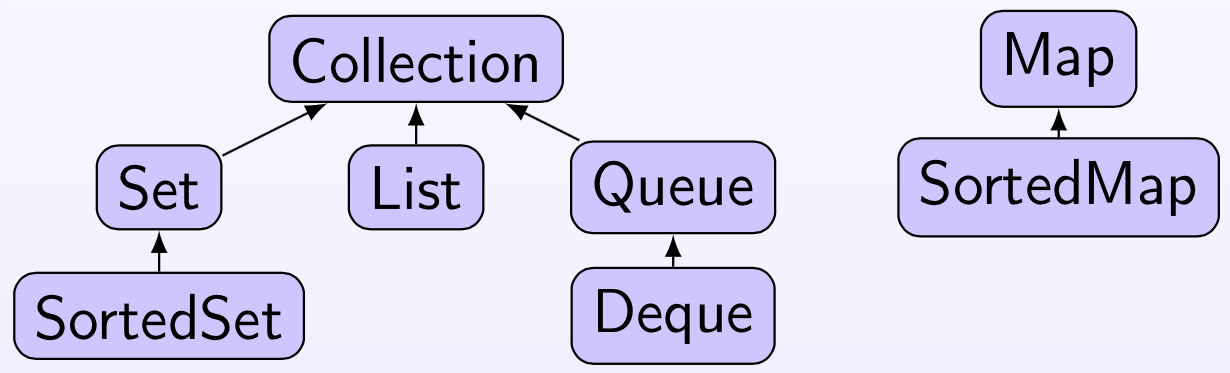
\includegraphics[width=0.5\textwidth]{colls-coreInterfaces.png}
    \label{Fig:collections}
  \caption{Interfacce del  Java collection framework.}
\end{figure}

Ogni interfaccia \`e generica. Quando dichiari una collezione devi specificare il tipo degli oggetti contenuti nella collezione. Questo permette al compilatore di verificare \textbf{a compile time} che l'oggetto che inserisci all'interno delle collezioni \`e corretto. 
\begin{lstlisting}
public interface Collection<E>...
\end{lstlisting}
Di seguito vengono specificate le interfacce principali
\begin{itemize}
\item \texttt{Collection}: una collezione rappresenta un gruppo di oggetti (i suoi elementi). L'interfaccia collection \`e la pi\`u generale. Va utilizzata quando un livello massimo di generalit\`a \`e richiesto. Alcuni tipi di collezioni consentono elementi duplicati, altri no, alcune sono ordinate altre no etc.  Non esiste una classe cheimplementa direttamente collection. Le classi implementano specifiche sottointerfacce come set liste etc. 
\item \texttt{Set}: una collezione che \textbf{non} pu\`o contenere elementi duplicati. Consente di modellare entit\`a come per esempio un mazzo di carte da briscola (perch\`e non \`e adatto per un mazzo di carte da scala?) l'insieme di esami sostenuti da uno studente, i processi in esecuzione su una macchina. 
\item \texttt{SortedSet}: un \texttt{Set} che mantiene gli elementi ordinati in ordine ascendente.  I \texttt{SortedSet} possono essere utilizzati (per esempio) per memorizzare una lista ordinata di parole.
\item \texttt{List}: \`e una collezione ordinata (a volte chiamata sequenza). Una lista pu\`o contenere elementi duplicati. L'utilizzatore di una lista vuole un controlllo periso su dove un elemento \`e inserito e vuole potervi accedere in base alla loro posizione. Pu\`o essere utile per esempio al fine di modellizzare l'ordine di arrivo a un gran premio di formula 1.
\item \texttt{Queue}: \`e una collezione utilizzata per modellizzare una coda di elementi  prima che vengano processati. Una coda \`e in genere implementata (ma non necessariamente) per mezzo di una coda di tipo FIFO (first-in, first-out). Consente di eseguire operazioni come l'inserimento, l'estrazione o l'ispezione. Una coda pu\`o essere utilizzata per modellare l'insieme di macchine in coda a un casello autostradale.
\item \texttt{Deque}: viene utilizzata per modellizzare una coda di elementi prima che vengano processati. A differenza della coda, \`e possibile aggiungere e rimuovere gli elementi da entrambi i lati.
\item \texttt{Map}: \`e un oggetto che mappa una chiave in un valore. Una mappa \textbf{non} pu\`o contenere delle chiavi duplicate, ogni chiave deve essere associata a esattamente un valore (che potrebbe essere un \textbf{Set}). 
\item \texttt{SortedMap}: contiene una mappa dove le chiavi sono mantenute in ordine ascendente. Per esempio le mappe ordinate possono essere utilizzate per modellizzare un vocabolario o una guida telefonica.
\end{itemize}


Per ogni interfaccia ci sono un insieme di possibili \textbf{implementazioni}. In particolare abbiamo varie implementazioni per vari contesti, tra le quali:
\begin{itemize}
\item \texttt{Implementazioni General-purpose} sono quelle comunemente utilizzate, progettate per l'uso di tutti i giorni
\item \texttt{Implementazioni Special-purpose} sono progettati per usi particolari: garantire performances particolari, restringere l'utilizzo di quelle general purpose.
\item \texttt{Concurrent implementations} sono progettate per supportare applicazioni concorrenti. Queste implementazioni fanno parte del  java.util.concurrent package.
\item \texttt{Wrapper implementations} sono utilizzate in combinazioni con altri tipi di implementazioni per fornire funzionalit\`a aggiunte o ristette.
\end{itemize}

Le implementazioni General-purpose sono schematizzate nella tabella seguente 

\begin{tabular}{ | l | l | l | l | l | l |}
\hline
  Interfaces & Hash table  & Resizable array  & Tree  & Linked list  & Hash table + Linked list  \\
  \hline
  \texttt{Set} & \texttt{HashSet} &  & \texttt{TreeSet} && \texttt{LinkedHashSet} \\
  \hline
    \texttt{SortedSet} & &  & \texttt{TreeSet} &&  \\
  \hline
  \texttt{List} &  & \texttt{ArrayList}  & & \texttt{LinkedList} & \\
\hline  
  \texttt{Queue} &  & & & \texttt{LinkedList} &  \\
\hline  
  \texttt{Deque} &  & \texttt{ArrayDeque} & & \texttt{LinkedList} & \\
\hline  
  \texttt{Map} & \texttt{HashMap} & & \texttt{TreeMap} && \texttt{LinkedHashMap} \\
  \hline
    \texttt{SortedMap} & & & \texttt{TreeMap} &&  \\
\hline    
\end{tabular} 

Ognuna di queste implementazioni:
\begin{itemize}
\item permette elementi \texttt{null} (sia per chiavi che per valori)
\item non \`e sincronizzata (thread-safe): non adatta quando thread concorrenti devono modificare la collezione
\item ha degli itaratori \emph{fail-fast} lanciano un eccezione quando viene eseguita una modica durante un iterazione. 
\item sono tutte serializzabili
\item hanno tutte un metodo clone (nota il metodo clone non clona gli elementi ma solo i loro references)
\end{itemize}

\begin{framed}
Come regola \`e bene pensare in termini di interfacce e non di implementazioni. Nella maggior parte dei casi l'implementazione influenza solo le performances. E\` bene associare un implementazione direttamente alla sua interfaccia e specificare come parametri di ingresso o uscita dei metodi solamente interfacce, lasciando il programmatore libero di cambiare implementazione a suo piacimento. 
\end{framed}




\section{Esercizi}

\subsection{Tipo statico e tipo dinamico}
\subsubsection{Esercizio 1}
Dire cosa stampa il seguente programma 
\begin{lstlisting}[language=Java,escapechar=|]
public static void main(String[] args) {
		ClassA a1, a2;
		ClassB b1;
		ClassC c1;

		a1 = new ClassB();
		b1 = new ClassB();
		c1 = new ClassC();
		a2 = new ClassC();

		/*
		 * b1 e' di classe ClassB, viene chiesto di invocare il metodo stampa su
		 * un parametro b1 di tipo statico ClassB. A compile scelgo la signature
		 * "compatibile" e piu' "vicina", considerando i tipi statici delle
		 * variabili. In particolare in questo caso la signature scelta e'
		 * public void stampa(ClassB p).
		 * 
		 * A run time b1 e' di classe classB e e il parametro p, che equivale a
		 * B1 e' anch'esso di classe ClassB per cui viene chiamato il metodo
		 * public void stampa(ClassB p) di class B (stampa BBB)
		 */
		b1.stampa(b1);
		/*
		 * a1 e' di classe ClassA, viene chiesto di invocare il metodo stampa su
		 * un parametro b1 di tipo statico ClassB. A compile scelgo la signature
		 * "compatibile" e piu' "vicina", considerando i tipi statici delle
		 * variabili. In particolare in questo caso la signature scelta e'
		 * public void stampa(ClassA p) della classe ClassA.
		 * 
		 * A run-time a1 e' di classe ClassB. Per questo partendo da classB e
		 * risalendo nella gerarchia di raffinamento cerco un metodo che matchi
		 * la signature public void stampa(ClassA p). In questo caso il metodo
		 * e' gia' presente in ClassB. Quindi viene invocato il metodo public
		 * void stampa(ClassA p) della classe ClassB (Stampa AAA/BBB)
		 */
		a1.stampa(b1);

		/*
		 * b1 e' di classe ClassB, viene chiesto di invocare il metodo stampa su
		 * un parametro c1 di tipo statico ClassC. A compile scelgo la signature
		 * "compatibile" e piu' "vicina", considerando i tipi statici delle
		 * variabili (ClassB). In particolare in questo caso la signature scelta
		 * all'interno di ClassB e' public void stampa(ClassA p) della classe
		 * ClassB.
		 * 
		 * A run-time b1 e' di classe ClassB, c1 e' di classe ClassC. Per questo
		 * partendo da classB e risalendo nella gerarchia di raffinamento cerco
		 * un metodo che matchi la signature public void stampa(ClassA p). In
		 * questo caso il metodo e' gia' presente in ClassB. Quindi viene
		 * invocato il metodo public void stampa(ClassA p) della classe ClassB
		 * (Stampa AAA/BBB)
		 */
		b1.stampa(c1);

		/*
		 * c1 e' di classe statica ClassC, viene chiesto di invocare il metodo stampa su
		 * un parametro c1 di tipo statico ClassC. A compile scelgo la signature
		 * "compatibile" e piu' "vicina", considerando i tipi statici delle
		 * variabili (ClassC). In particolare in questo caso la signature scelta
		 * all'interno di ClassC e' public void stampa(ClassC p) della classe
		 * ClassC.
		 * 
		 * A run-time c1 e' di classe ClassC, c1 e' di classe ClassC. Per questo
		 * partendo da ClassC e risalendo nella gerarchia di raffinamento cerco
		 * un metodo che matchi la signature public void stampa(ClassC p). In
		 * questo caso il metodo e' gia' presente in ClassC. Quindi viene
		 * invocato il metodo public void stampa(ClassC p) della classe ClassC
		 * (Stampa CCC)
		 */
		c1.stampa(c1);
		
		/*
		 * c1 e' di classe statica ClassC, viene chiesto di invocare il metodo stampa su
		 * un parametro a1 di tipo statico ClassA. A compile scelgo la signature
		 * "compatibile" e piu' "vicina", considerando i tipi statici delle
		 * variabili. In particolare in questo caso la signature scelta
		 * all'interno di ClassC e' public void stampa(ClassA p) della classe
		 * ClassC.
		 * 
		 * A run-time c1 e' di classe ClassC, a1 e' di classe ClassB. Per questo
		 * partendo da ClassC e risalendo nella gerarchia di raffinamento cerco
		 * un metodo che matchi la signature public void stampa(ClassA p). In
		 * questo caso il metodo e' gia' presente in ClassC. Quindi viene
		 * invocato il metodo public void stampa(ClassA p) della classe ClassC
		 * (Stampa AAA/CCC)
		 */
		c1.stampa(a1);

		/*
		 * a2 e' di classe statica ClassA, viene chiesto di invocare il metodo stampa su
		 * un parametro c1 di tipo statico ClassC. A compile scelgo la signature
		 * "compatibile" e piu' "vicina", considerando i tipi statici delle
		 * variabili. In particolare in questo caso la signature scelta
		 * all'interno di ClassA e' public void stampa(ClassA p) della classe
		 * ClassA.
		 * 
		 * A run-time a2 e' di classe ClassC, c1 e' di classe ClassC. Per questo
		 * partendo da ClassC e risalendo nella gerarchia di raffinamento cerco
		 * un metodo che matchi la signature public void stampa(ClassA p). In
		 * questo caso il metodo e' gia' presente in ClassC. Quindi viene
		 * invocato il metodo public void stampa(ClassA p) della classe ClassC
		 * (Stampa AAA/CCC)
		 */
		a2.stampa(c1);
	}
\end{lstlisting}
dove 
\begin{lstlisting}[language=Java,escapechar=|]
public class ClassA {

	public void stampa(ClassA p){
		System.out.println("AAA");
	}
}
\end{lstlisting}

\begin{lstlisting}[language=Java,escapechar=|]
public class ClassB extends ClassA {
	public void stampa(ClassB p){
		System.out.println("BBB");
	}
	public void stampa(ClassA p){
		System.out.println("AAA/BBB");
	}
}
\end{lstlisting}

\begin{lstlisting}[language=Java,escapechar=|]
public class ClassC extends ClassA {
	public void stampa(ClassC p){
		System.out.println("CCC");
	}
	public void stampa(ClassA p){
		System.out.println("AAA/CCC");
	}
}
\end{lstlisting}

\subsubsection{Esercizio 2}
\begin{framed}
\textbf{Esercizio 6a}: Cosa succede se \texttt{ClassC} eredita da \texttt{ClassB} e non da \texttt{ClassA}
\end{framed}
\begin{lstlisting}[language=Java,escapechar=|]
package tipostaticoedinamico;

public class Main {

	public static void main(String[] args) {
		ClassA a1, a2;
		ClassB b1;
		ClassC c1;

		a1 = new ClassB();
		b1 = new ClassB();
		c1 = new ClassC();
		a2 = new ClassC();

		/*
		 * b1 e' di classe ClassB, viene chiesto di invocare il metodo stampa su
		 * un parametro b1 di tipo statico ClassB. A compile scelgo la signature
		 * "compatibile" e piu' "vicina", considerando i tipi statici delle
		 * variabili. In particolare in questo caso la signature scelta e'
		 * public void stampa(ClassB p).
		 * 
		 * A run time b1 e' di classe classB e e il parametro p, che equivale a
		 * B1 e' anch'esso di classe ClassB per cui viene chiamato il metodo
		 * public void stampa(ClassB p) di class B (stampa BBB)
		 */
		b1.stampa(b1);
		/*
		 * a1 e' di classe ClassA, viene chiesto di invocare il metodo stampa su
		 * un parametro b1 di tipo statico ClassB. A compile scelgo la signature
		 * "compatibile" e piu' "vicina", considerando i tipi statici delle
		 * variabili. In particolare in questo caso la signature scelta e'
		 * public void stampa(ClassA p) della classe ClassA.
		 * 
		 * A run-time a1 e' di classe ClassB. Per questo partendo da classB e
		 * risalendo nella gerarchia di raffinamento cerco un metodo che matchi
		 * la signature public void stampa(ClassA p). In questo caso il metodo
		 * e' gia' presente in ClassB. Quindi viene invocato il metodo public
		 * void stampa(ClassA p) della classe ClassB (Stampa AAA/BBB)
		 */
		a1.stampa(b1);

		/*
		 * b1 e' di classe ClassB, viene chiesto di invocare il metodo stampa su
		 * un parametro c1 di tipo statico ClassC. A compile scelgo la signature
		 * "compatibile" e piu' "vicina", considerando i tipi statici delle
		 * variabili (ClassB). In particolare in questo caso la signature scelta
		 * all'interno di ClassB e' public void stampa(ClassB p) della classe
		 * ClassB.
		 * 
		 * A run-time b1 e' di classe ClassB, c1 e' di classe ClassC. Per questo
		 * partendo da classB e risalendo nella gerarchia di raffinamento cerco
		 * un metodo che matchi la signature public void stampa(ClassB p). In
		 * questo caso il metodo e' gia' presente in ClassB. Quindi viene
		 * invocato il metodo public void stampa(ClassB p) della classe ClassB
		 * (Stampa BBB)
		 */
		b1.stampa(c1);

		/*
		 * c1 e' di classe statica ClassC, viene chiesto di invocare il metodo stampa su
		 * un parametro c1 di tipo statico ClassC. A compile scelgo la signature
		 * "compatibile" e piu' "vicina", considerando i tipi statici delle
		 * variabili (ClassC). In particolare in questo caso la signature scelta
		 * all'interno di ClassC e' public void stampa(ClassC p) della classe
		 * ClassC.
		 * 
		 * A run-time c1 e' di classe ClassC, c1 e' di classe ClassC. Per questo
		 * partendo da ClassC e risalendo nella gerarchia di raffinamento cerco
		 * un metodo che matchi la signature public void stampa(ClassC p). In
		 * questo caso il metodo e' gia' presente in ClassC. Quindi viene
		 * invocato il metodo public void stampa(ClassC p) della classe ClassC
		 * (Stampa CCC)
		 */
		c1.stampa(c1);
		
		/*
		 * c1 e' di classe statica ClassC, viene chiesto di invocare il metodo stampa su
		 * un parametro a1 di tipo statico ClassA. A compile scelgo la signature
		 * "compatibile" e piu' "vicina", considerando i tipi statici delle
		 * variabili. In particolare in questo caso la signature scelta
		 * all'interno di ClassC e' public void stampa(ClassA p) della classe
		 * ClassC.
		 * 
		 * A run-time c1 e' di classe ClassC, a1 e' di classe ClassB. Per questo
		 * partendo da ClassC e risalendo nella gerarchia di raffinamento cerco
		 * un metodo che matchi la signature public void stampa(ClassA p). In
		 * questo caso il metodo e' gia' presente in ClassC. Quindi viene
		 * invocato il metodo public void stampa(ClassA p) della classe ClassC
		 * (Stampa AAA/CCC)
		 */
		c1.stampa(a1);

		/*
		 * a2 e' di classe statica ClassA, viene chiesto di invocare il metodo stampa su
		 * un parametro c1 di tipo statico ClassC. A compile scelgo la signature
		 * "compatibile" e piu' "vicina", considerando i tipi statici delle
		 * variabili. In particolare in questo caso la signature scelta
		 * all'interno di ClassA e' public void stampa(ClassA p) della classe
		 * ClassA.
		 * 
		 * A run-time a2 e' di classe ClassC, c1 e' di classe ClassC. Per questo
		 * partendo da ClassC e risalendo nella gerarchia di raffinamento cerco
		 * un metodo che matchi la signature public void stampa(ClassA p). In
		 * questo caso il metodo e' gia' presente in ClassC. Quindi viene
		 * invocato il metodo public void stampa(ClassA p) della classe ClassC
		 * (Stampa AAA/CCC)
		 */
		a2.stampa(c1);
	}
}
\end{lstlisting}

\subsubsection{Esercizio 3}
Dire cosa stampa il seguente programma 
\begin{lstlisting}[language=Java,escapechar=|]
public class Main {

	public static void main(String[] args) {
		Figura f1, f2;
		Quadrato q=new Rettangolo();
		Rettangolo r=new Rettangolo();
		f1=new Quadrato();
		f2=new Rettangolo();
		
		/*
		 * f1 e' di classe statica Figura, viene chiesto di invocare il metodo stampa su
		 * un parametro f2 di tipo statico Figura. A compile scelgo la signature
		 * "compatibile" e piu' "vicina", considerando i tipi statici delle
		 * variabili. In particolare in questo caso la signature scelta
		 * all'interno di Figura e' public void stampa(Figura p) della classe
		 * Figura.
		 * 
		 * A run-time f1 e' di classe Quadrato, f2 e' di classe Rettangolo. Per questo
		 * partendo da Quadrato e risalendo nella gerarchia di raffinamento cerco
		 * un metodo che matchi la signature public void stampa(Figura p). In
		 * questo caso il metodo e' presente solo in Figura. Quindi viene
		 * invocato il metodo public void stampa(Figura p) della classe Figura
		 * (Stampa Figura)
		 */
		f1.stampa(f2);
		
		/*
		 * q e' di classe statica Quadrato, viene chiesto di invocare il metodo stampa su
		 * un parametro r di tipo statico Rettangolo. A compile scelgo la signature
		 * "compatibile" e piu' "vicina", considerando i tipi statici delle
		 * variabili. In particolare in questo caso la signature scelta
		 * all'interno di Quadrato e' public void stampa(Rettangolo p) della classe
		 * Quadrato.
		 * 
		 * A run-time q e' di classe Rettangolo, r e' di classe Rettangolo. Per questo
		 * partendo da Rettangolo e risalendo nella gerarchia di raffinamento cerco
		 * un metodo che matchi la signature public void stampa(Rettangolo p). In
		 * questo caso il metodo e' presente in Rettangolo. Quindi viene
		 * invocato il metodo public void stampa(Rettangolo p) della classe Rettangolo
		 * (Stampa Rettangolo Particolare)
		 */
		q.stampa(r);
		
		/*
		 * f1 e' di classe statica Figura, viene chiesto di invocare il metodo stampa su
		 * un parametro q di tipo statico Quadrato. A compile scelgo la signature
		 * "compatibile" e piu' "vicina", considerando i tipi statici delle
		 * variabili. In particolare in questo caso la signature scelta
		 * all'interno di Figura e' public void stampa(Figura p) della classe
		 * Figura.
		 * 
		 * A run-time f1 e' di classe Quadrato, q e' di classe Rettangolo. Per questo
		 * partendo da Quadrato e risalendo nella gerarchia di raffinamento cerco
		 * un metodo che matchi la signature public void stampa(Figura p). In
		 * questo caso il metodo e' presente in Figura. Quindi viene
		 * invocato il metodo public void stampa(Figura p) della classe Figura
		 * (Stampa Figura)
		 */
		f1.stampa(q);
		
		/*
		 * q e' di classe statica Quadrato, viene chiesto di invocare il metodo stampa su
		 * un parametro f1 di tipo statico Figura. A compile scelgo la signature
		 * "compatibile" e piu' "vicina", considerando i tipi statici delle
		 * variabili. In particolare in questo caso la signature scelta
		 * all'interno di Quadrato e' public void stampa(Figura q) della classe
		 * Figura.
		 * 
		 * A run-time q e' di classe Rettangolo, f1 e' di classe Quadrato. Per questo
		 * partendo da Rettangolo e risalendo nella gerarchia di raffinamento cerco
		 * un metodo che matchi la signature public void stampa(Figura p). In
		 * questo caso il metodo e' presente in Rettangolo. Quindi viene
		 * invocato il metodo public void stampa(Figura p) della classe Rettangolo
		 * (Stampa Figura particolare)
		 */
		q.stampa(f1);
		
		/*
		 * q e' di classe statica Quadrato, viene chiesto di invocare il metodo stampa su
		 * un parametro q di tipo statico Quadrato. A compile scelgo la signature
		 * "compatibile" e piu' "vicina", considerando i tipi statici delle
		 * variabili. In particolare in questo caso la signature scelta
		 * all'interno di Quadrato e' public void stampa(Quadrato q) della classe
		 * Quadrato.
		 * 
		 * A run-time q e' di classe Rettangolo. Per questo
		 * partendo da Rettangolo e risalendo nella gerarchia di raffinamento cerco
		 * un metodo che matchi la signature public void stampa(Quadrato p). In
		 * questo caso il metodo e' presente in Rettangolo. Quindi viene
		 * invocato il metodo public void stampa(Quadrato p) della classe Rettangolo
		 * (Stampa Rettangolo particolare)
		 */
		q.stampa(q);

	}
}
\end{lstlisting}

Dove
\begin{lstlisting}[language=Java,escapechar=|]
public class Figura {
	public void stampa(Figura f){
		System.out.println("Figura");
	}
}
\end{lstlisting}
\begin{lstlisting}[language=Java,escapechar=|]
public class Quadrato extends Figura {
	public void stampa(Quadrato q){
		System.out.println("Quadrato");
	}
}
\end{lstlisting}
\begin{lstlisting}[language=Java,escapechar=|]
public class Rettangolo extends Quadrato {
	public void stampa(Rettangolo q) {
		System.out.println("Rettangolo");
	}

	public void stampa(Quadrato q) {
		System.out.println("Rettangolo particolare");
	}

	public void stampa(Figura q) {
		System.out.println("Figura particolare");
	}
}
\end{lstlisting}

\subsection{Casting di tipo}

\subsection{HashCode e Equals}
\subsection{Generics}
\subsubsection{Generic classes}
\begin{framed}
\textbf{Esercizio }: Pregettare la classe \texttt{Box}. La classe \texttt{Box} contiene un oggetto e fornisce il metodo \texttt{set}, che modifica l'oggetto contenuto nel box, e  \texttt{get}, che ottiene l'oggetto contenuto nel \texttt{Box}.
\end{framed}

\begin{lstlisting}[language=Java]
public class Box {
    private Object object;

    public void set(Object object) { this.object = object; }
    public Object get() { return object; }
}
\end{lstlisting}
Dal momento che i metodi accettano e ritornano un oggetto di tipo \texttt{Object}, l'utente \`e libero di passare qualunque dato non sia primitivo. Non c'\`e modo di verificare a \emph{compile time} come la classe viene usata. Per esempio un potrebbe usare in una parte di codice il Box come un box di interi, ma poit ``dimenticarsene" e in un altra parte passagli una stringa. Tale comportamento genera un errore a \emph{run time}. Per esempio il seguente snapshot genera un errore a run-time 
\begin{lstlisting}[language=Java]
public class Main {

	public static void main(String[] args) {
		Box b1=new Box();
		b1.set("1");
		String stringNumber=(String) b1.get();
		int number=(int) b1.get();
	}
}
\end{lstlisting}
In seguito viene descritta l'implementazione del box eseguita mediante l'utilizzo dei generici. Specifichiamo che la classe pu\`o contenere oggetti di un tipo \emph{generico} \texttt{T}. 

\begin{lstlisting}[language=Java]
/*
 * Generic version of the Box class.
 * @param <T> the type of the value being boxed
 */
public class Box<T> {
    // T stands for "Type"
    private T t;

    public void set(T t) { this.t = t; }
    public T get() { return t; }
}
\end{lstlisting}
Nel seguito viene descritto un possibile utilizzo della classe \texttt{Box}, un \texttt{Box} contenente una stringa. Analogamente \`e possibile dichiarare un \texttt{Box} contenente una bicicletta come \texttt{Box<Bicicletta>}.
\begin{lstlisting}[language=Java]
public class Main {

	public static void main(String[] args) {
		Box<String> b1=new Box<String>();
		b1.set("1");
		b1.set(1); // errore a compile time
		String stringNumber= b1.get();
		int number=b1.get(); // errore a compile time
	}
}
\end{lstlisting}

\subsubsection{Generic methods}
\begin{framed}
\textbf{Esercizio }: Pregettare una classe \texttt{Utils}, contenente un metodo che dati due \texttt{Box} ritorna \texttt{true} se entrambi i box sono vuoti, \texttt{false} altrimenti.
\end{framed}
Prima di tutto aggiungiamo il metodo \texttt{isEmpty()} alla classe box
\begin{lstlisting}[language=Java]
public boolean isEmpty(){
    		return (t==null);
    }
\end{lstlisting}

Definiamo il metodo \texttt{check} i cui parametri sono due \texttt{Box} che contengono un elemento di tipo \texttt{K} e \texttt{V}, rispettivamente, il cui comportamento rispetta i requisiti richiesti.
\begin{lstlisting}[language=Java]
public final class Utils {

	public static <T1, T2>  boolean check(Box<T1> box1, Box<T2> box2){
		return box1.isEmpty()&&box2.isEmpty();
	}
}
\end{lstlisting}
Specifichiamo un client che utilizza il metodo \texttt{check}
\begin{lstlisting}[language=Java]
public class Main {

	public static void main(String[] args) {
		Box<String> b1=new Box<String>();
		b1.set("1");
		Box<String> b2=new Box<String>();
		b2.set("1");
		Box<Integer> b3=new Box<Integer>();
		Box<String> b4=new Box<String>();
		System.out.println(Utils.<String, String>check(b1, b2));
		System.out.println(Utils.<String, String>check(b1, b2));
		System.out.println(Utils.<Integer, String>check(b3, b4));
	}
}
\end{lstlisting}

\subsubsection{Generic Bounded types}
\begin{framed}
\textbf{Esercizio }: Pregettare la classe \texttt{Box}. La classe \texttt{Box} contiene un oggetto di tipo \textbf{animale} o suoi sottotipi. La classe fornisce il metodo \texttt{set}, che modifica l'oggetto contenuto nel box, e  \texttt{get}, che ottiene l'oggetto contenuto nel \texttt{Box}.
\end{framed}
E\` possibile specificare che il tipo generico sostituito a \texttt{T} debba estendere una classe o implementare un interfaccia. Nel caso in questione forziamo \texttt{T} a estendere la classe \texttt{Animale}.

\begin{lstlisting}[language=Java]
/*
 * Generic version of the Box class.
 * @param <T> the type of the value being boxed
 */
public class Box<T extends Animale> {
    // T stands for "Type"
    private T t;

    public void set(T t) { this.t = t; }
    public T get() { return t; }
    
    public boolean isEmpty(){
    		return (t==null);
    }
}
\end{lstlisting}

Di seguito viene specificato un client per la nuova classe \texttt{Box}

\begin{lstlisting}[language=Java]
public class Main {

	public static void main(String[] args) {
		Box<Animale> b1=new Box<Animale>();
		b1.set(new Cane());
		System.out.println(b1.get());
		Box<String> b2=new Box<String>(); // ERRORE COMPILAZIONE
	}
}
\end{lstlisting}



\subsection{Collezioni}
\subsubsection{Liste assegnamenti}
\begin{framed}
\textbf{Esercizio }: Dire se sono valide le seguenti operazioni
\begin{lstlisting}
List<String> ls=new ArrayList<String>();
List<Object> lo=ls;
\end{lstlisting}
\end{framed}

\begin{lstlisting}
List<String> ls=new ArrayList<String>(); // certamente si
List<Object> lo=ls;    //no, il compilatore non lo permette
\end{lstlisting}

\subsubsection{Collection Print}
\begin{framed}
\textbf{Esercizio }: Scrivere un metodo che stampa gli elementi di una collection di qualsiasi tipo
\end{framed}

\begin{lstlisting}
void printCollection(Collection<Object> c){
    for(Object e: c){
        System.out.println(e);     
     }   
}
\end{lstlisting}


\subsubsection{Rimozione di duplicati}
\begin{framed}
\textbf{Esercizio }: Scrivere un metodo statico che data una collezione di \texttt{String} rimuove i duplicati e stampa il numero di elementi non duplicati e i corrispettivi elementi
\end{framed}

Nella prima versione della soluzione utilizziamo il for generalizzato
\begin{lstlisting}
package es1;

import java.util.ArrayList;
import java.util.Collection;
import java.util.HashSet;
import java.util.List;
import java.util.Scanner;
import java.util.Set;

public class FindDups {
	public static void findDups(Collection<String> words){
		Set<String> set = new HashSet<String>();
		for (String s: words){
			set.add(s);
		}
		System.out.println("Unique values, dim : " + 
		set.size() + " Elements:" + set);
			
	}
}
\end{lstlisting}

Nella seconda versione utilizziamo direttamente il costruttore di \texttt{HashSet} vedi (\url{https://docs.oracle.com/javase/6/docs/api/java/util/HashSet.html})
\begin{lstlisting}
package collections;

import java.util.Collection;
import java.util.HashSet;
import java.util.Set;

public class FindDups {
	public static void findDups(Collection<String> words){
		Set<String> set = new HashSet<String>(words);
		System.out.println("Unique values, dim : " + 
				set.size() + " Elements:" + set);
		
	}
}

\end{lstlisting}
Di seguito viene riportato un client per la classe \texttt{FindDups}.
\begin{lstlisting}
	public static void main(String[] args){
		Scanner s = new Scanner(System.in);
		String word = null;
		System.out.println("Inserire le parole, (q per uscire)");
		List<String> words = new ArrayList<String>();
		word = s.nextLine();		
		while (!word.equals("q") ){
			words.add(word);
			word = s.nextLine();
		} 
		findDups(words);
		s.close();
	}
}
\end{lstlisting}

\subsubsection{Shuffle}
\begin{framed}
\textbf{Esercizio }: Scrivere un metodo statico che data una permette di mescolare degli oggetti contenuti in una lista.
\end{framed}
Nella prima versione implementiamo la funzione shuffle 
\begin{lstlisting}
package collections;

import java.util.List;
import java.util.Random;

public class Shuffle {
	public static <E> void swap(List<E> a, int i, int j) {
		    E tmp = a.get(i);
		    a.set(i, a.get(j));
		    a.set(j, tmp);
	}
	
	public static void shuffle(List<Integer> list, Random rnd) {
		    for (int i = list.size(); i > 1; i--)
		        swap(list, i - 1, rnd.nextInt(i));
	}
}
\end{lstlisting}
Ecco il corrispettivo client
\begin{lstlisting}
public class Main {

	public static void main(String[] args){
		List<Integer> list = new ArrayList<Integer>();
		for (int i = 0; i < 10; i++){
			list.add(i);
		}
		System.out.println(list);
		Shuffle.shuffle(list, new Random());
		System.out.println(list);
	}
}
\end{lstlisting}
Nella seconda versione utilizziamo il metodo \texttt{shuffle} contenuto nella classe \texttt{Collections}.

\begin{lstlisting}
public class Shuffle {
	public static void shuffle(List<Integer> list) {
		Collections.shuffle(list);
	}
}
\end{lstlisting}
Ecco il corrispondente client
\begin{lstlisting}
package collections;

import java.util.ArrayList;
import java.util.List;

public class Main {

	public static void main(String[] args){
		List<Integer> list = new ArrayList<Integer>();
		for (int i = 0; i < 10; i++){
			list.add(i);
		}
		System.out.println(list);
		Shuffle.shuffle(list);
		System.out.println(list);
	}
}
\end{lstlisting}





\subsection{Stack}



\subsubsection{Node}
\begin{lstlisting}
/**
* contiene un nodo dello stack. 
* Un nodo contiene un reference al prossimo nodo (next)
* e l'elemento corrente (element)
*/
class Node<E> {
    /**
    * contiene il reference al prossimo elemento
    */	
    Node<E> next;
    /**
    * contiene l'elemento contenuto nel nodo
    */
    E element;
}
\end{lstlisting}

\subsubsection{Stack}
\begin{lstlisting}
import java.util.Collection;

/**
* contiene l'interfaccia che definisce le operazioni consentite dallo stack
*/
public interface MyStack <E>{
    /**
    * rimuove un elemento dal top dello stack
    */
    public E pop();
    /**
    * inserisce un elemento nello stack
    */
    public void push(E elem);
    /**
    * ritorna vero se lo stack e' vuoto
    */
    public boolean isEmpty();
    /**
    * ritorna la dimensione dello stack
    */
    public int size();
    /**
    * ritorna vero se l'elemento e' contenuto nello stack
    */
    public boolean contains(E elem);
    /**
    * ritorna vero se lo stack contiene tutti gli elementi della collezione
    */
    public boolean containsAll(Collection<? extends E> collection);
}
\end{lstlisting}

\subsection{LinkedListStack}
\begin{lstlisting}
import java.util.Collection;

public class LinkedListStack<E> implements MyStack<E>{
	private int N;
	private Node<E> head;

	public LinkedListStack(){
		head = null;
		N = 0;
	}
	
	@Override
	public E pop() {
		if (isEmpty())
			return null;
		E elem = head.element;
		head = head.next;
		N--;
		return elem; 
	}

	@Override
	public void push(E elem) {
		Node<E> oldHead = head;
		head = new Node<E>();
		head.element = elem;
		head.next = oldHead;
		N++;		
	}

	@Override
	public boolean isEmpty() {		
		return N == 0;
	}

	@Override
	public boolean contains(E elem) {
		Node<E> tmp = head;
		while (tmp!= null){
			if (tmp.element.equals(elem))
				return true;
			tmp = tmp.next;
		}
		return false;
	}

	@Override
	public boolean containsAll(Collection<? extends E> collection) {		
		for (E elem: collection){
			if (!contains(elem))
				return false;			
		}
		return true;
	}
	
	@Override
	public int size(){
		return N;
	}
	
	public static <E> MyStack<E> createFromArray(E[] arr){
		MyStack<E>	stack = new LinkedListStack<>();
		for (E elem: arr){
			stack.push(elem);
		}
		return stack;
	}

	
	public static void main(String[] args){
		String [] arr = {"a","b","c","d"};
		MyStack<String> stack = createFromArray(arr);
		System.out.println(stack.contains("c"));
		System.out.println(stack.contains("f"));
		stack.push("e");
		while (!stack.isEmpty()){
			System.out.println(stack.pop());
		}
	}
}
\end{lstlisting}

\subsection{Esercizi per casa}
\begin{itemize}
\item Esercizio : generics
\begin{itemize}
\item implementare la classe coppia, che rappresenta una coppia di elementi. I due elementi hanno dei tipi generici \texttt{K}, \texttt{V}.
\item progettare un metodo statico che date due coppie i cui elementi sono dello stesso tipo titorna true se le coppie rappresentano il medesimo oggetto
\end{itemize} 
\end{itemize}

\clearpage

% ---- Bibliography ----




\addcontentsline{toc}{chapter}{Bibliography}
\bibliographystyle{alpha}
\bibliography{bib}
\nocite{*}


\end{document}

